\subsection{Memory Resistor}

%Robin.

Memory resistors, memsistors for short, are passive circuits which change their resistance as current flows through them, and maintain their resistance in between use. In other words, memsistors remember past flows of current (i.e. store state), and control resistance based on this knowledge (i.e. stored state). Several similarities have been identified bewteen the properties of memsistors and synapses, which make them interesting candidates for associative memory models.

TODO: Extend. Artificial synapses experiment using memsistors conducted in 2010, empiricially validating the formation of associative memories using three neurons and two synapses \cite{memristor_conditioning}.

TODO: Extend. The memsistor was hyphosized in 1972 by Leon Chua, the father of non-linear curcuit theory, who presented it as the missing fundamental cirtuit element (see figure \ref{fig:circuit_elements}) \cite{chua_memristor}. Looking at the current~$I$ and voltage~$V$ plot, a memsistor may be identified by the pinched hysteresis loop going through origo (see figure \ref{fig:pinched_hysteresis}. TODO: Explain the underlying reason of the hysteresis loop, i.e. alterating between two states (metastable switch).

% ref: Finding the Missing Memristor - R. Stanley Williams
%
% > The fourth fundamental passive circuit element.
% >
% > Resistor
% > Capacitor
% > Inductor
% >
% > AND Memristor
% >
% > UC Bercley Lean Chua is to circuit theory what Albert Einstein is to relativity.
% > The father of non-linear cirtuit theory.
% >
% > Noticed something missing from the circuit diagram; based on symmetry and beauty, there should be a fourth.
% > Original paper, memsitory the missing circuit element. 1971
% >
% > Passive device with state.
% >
% > Frequency response of Lissajous figures.
% > The pinched hysteresis loop.
% >
% > "If you see a pinced hysteresis loop in an IV-curve, you've probably got a memristor."
% >
% > Make a circuit using only resistors, capacitors and inductors to come up with the IV-characteristics of a memristor. It cannot be done, and thus belongs to it as a fundamental device; as proven by Lean Chua.
% >
% > Even before the original paper in 1971, there was peer-review research published which illustrated pinched hysteresis loop. Basically they had managed to discover the memristor, they just didn't know what it was called and thought it was an abnomality.
% >
% > Strukov, Stewart, Snider & Williams, Nature 453 80 (2008)

\begin{figure}[htbp]
	\begin{center}
		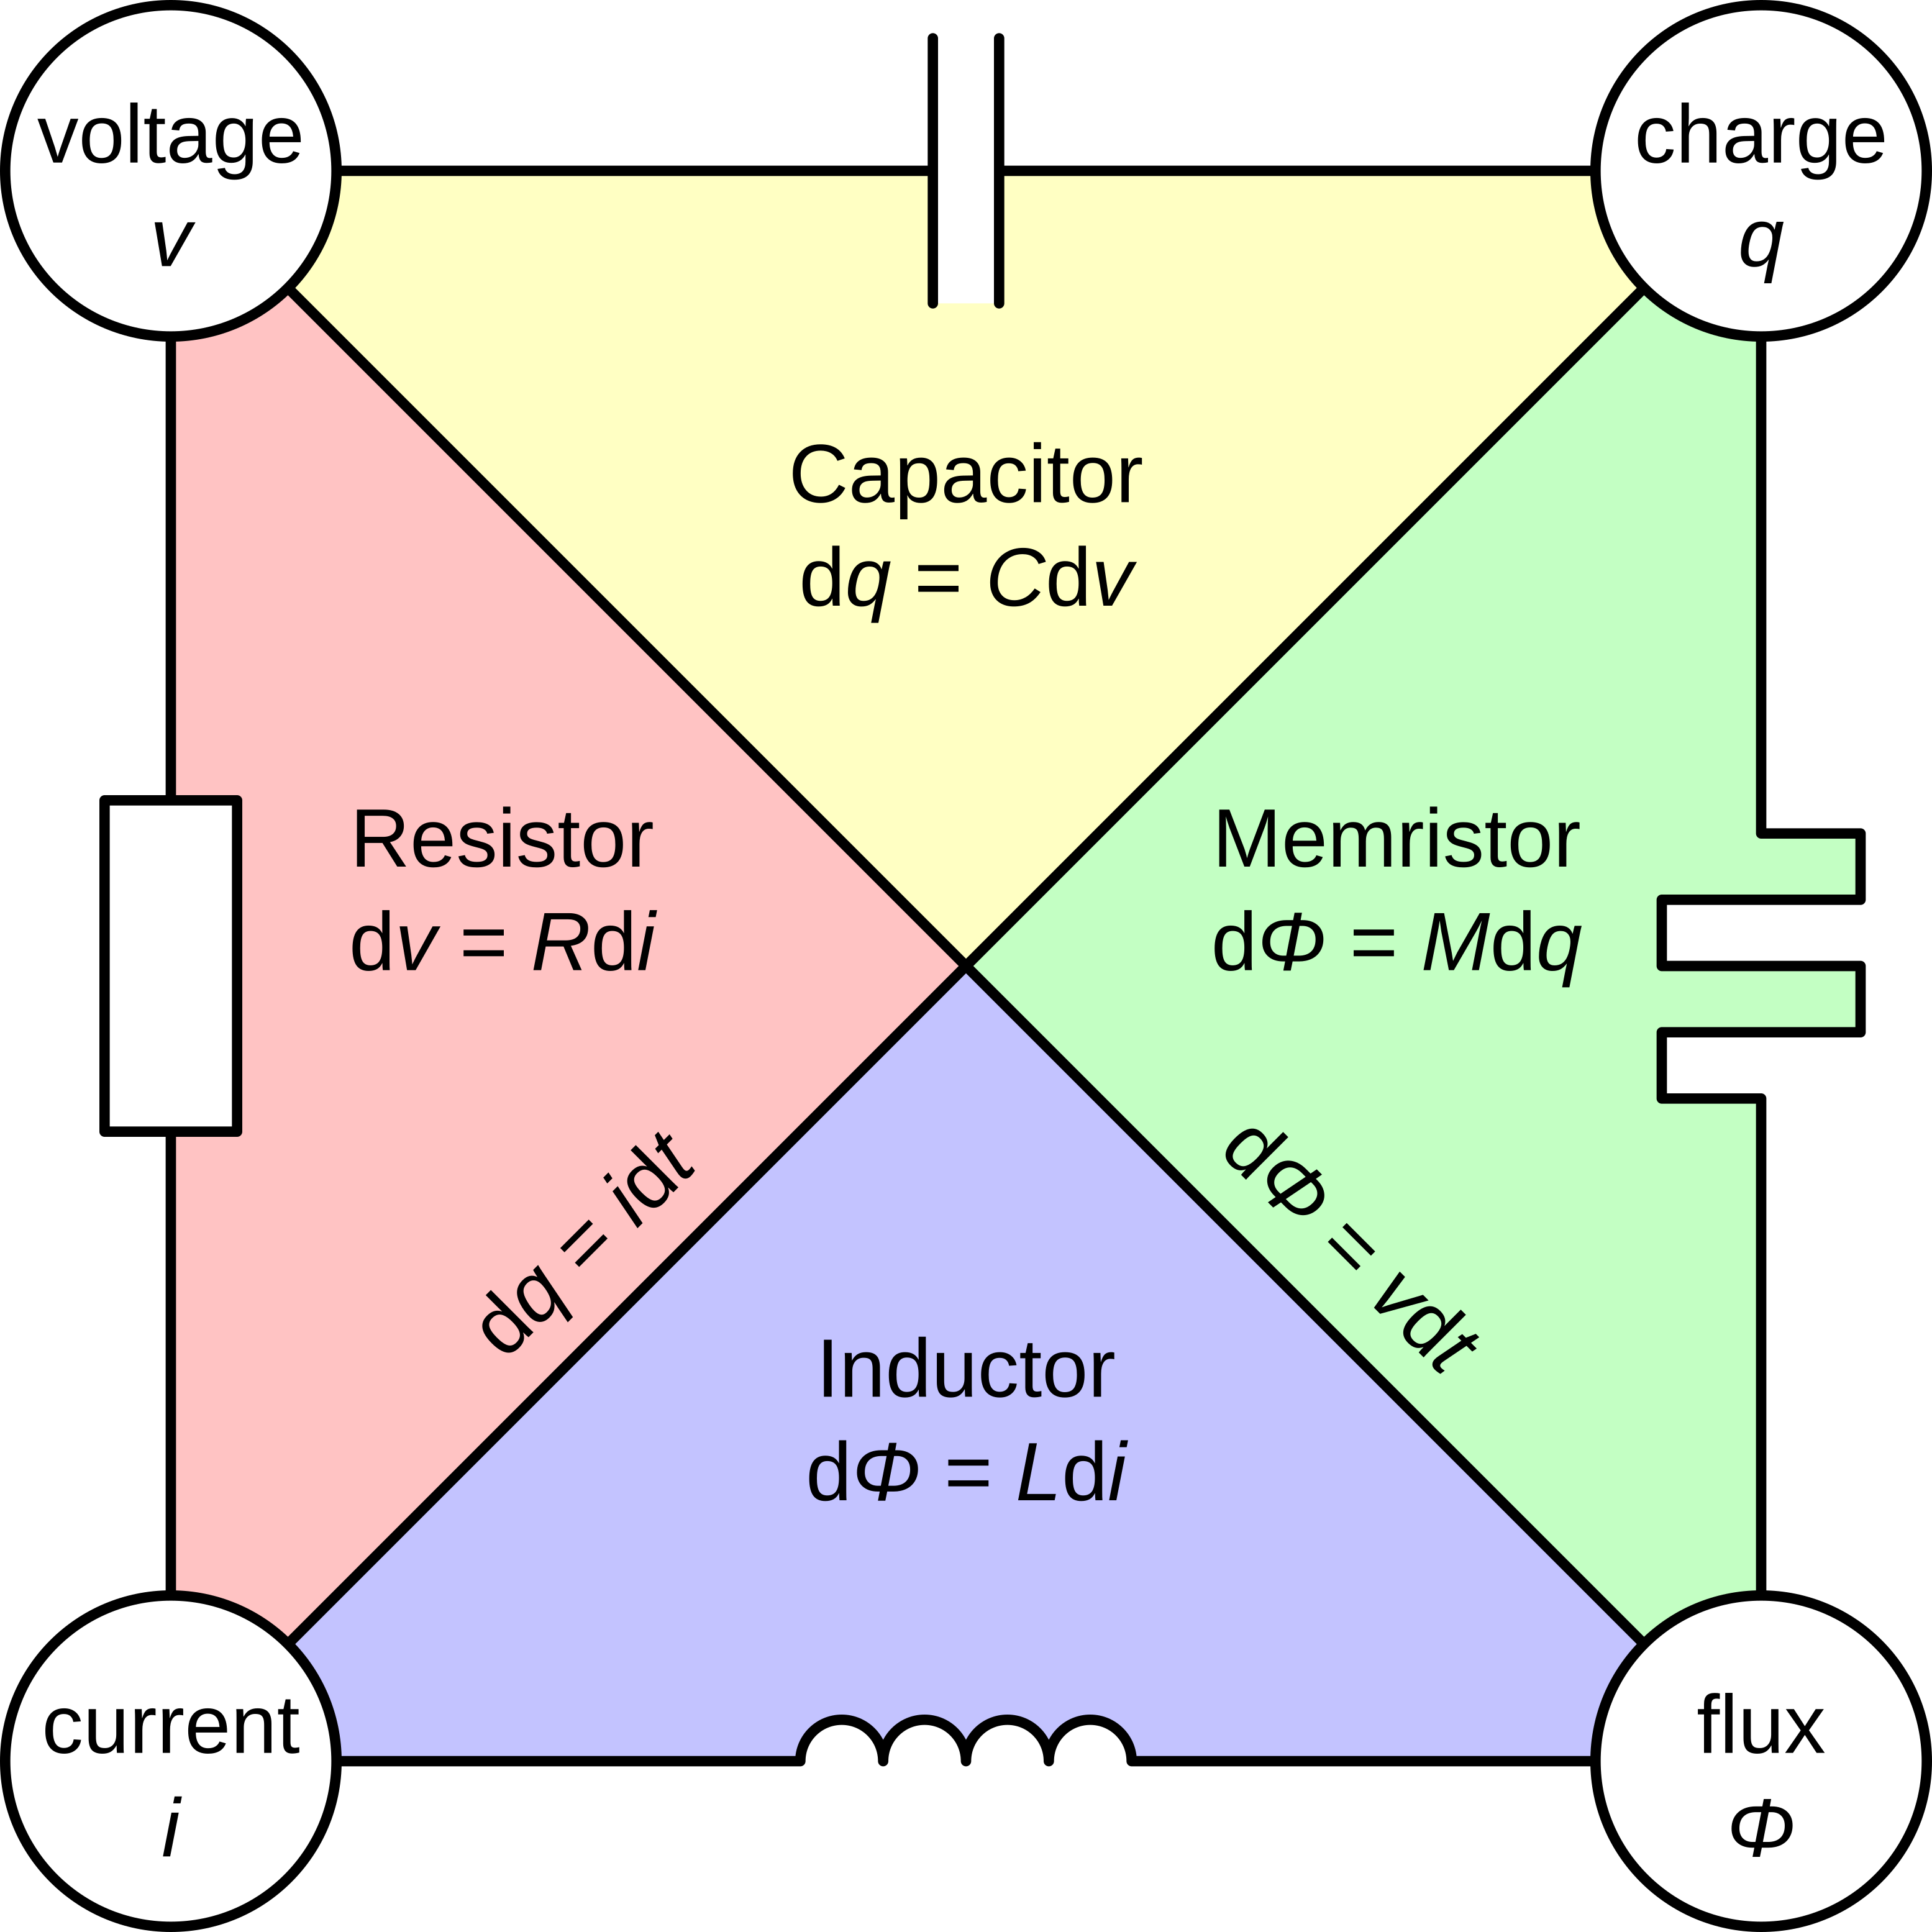
\includegraphics[width=0.5\textwidth]{inc/circuit_elements.png}
		\caption{Fundamental circuit elements.\protect\footnotemark}
		\label{fig:circuit_elements}
	\end{center}
\end{figure}
\footnotetext{Original image (CC BY-SA): \url{https://en.wikipedia.org/wiki/File:Two-terminal_non-linear_circuit_elements.svg}}

\begin{figure}[htbp]
	\begin{center}
		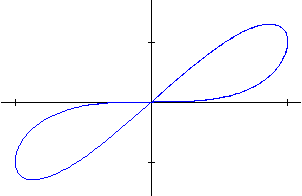
\includegraphics[width=0.5\textwidth]{inc/pinched_hysteresis.png}
		\caption{A pinched hysteresis loop plotted on an IV-curve.\protect\footnotemark}
		\label{fig:pinched_hysteresis}
	\end{center}
\end{figure}
\footnotetext{Original image (CC BY-SA): \url{https://en.wikipedia.org/wiki/File:Pinched_crossing_hysteresis.png}}

TODO: Extend. In 2008, HP released a paper titled \textit{The missing memristor found}, which outlined the hardware implementation of a memsistor \cite{hp_memristor_found}, thus validating the existence of the hypothesized memsistors circuit element. Retrospectively, several research groups had discovered circuits with the tell-tale properties of memsistor, i.e. with a pinched hysteresis loop. TODO: Include ref about prior research, before 2008.

% ref: Tim Molter HiPeac Prague 2016 Memristor Keynote
%
% The resistance of a memristor depends on the history of current that has previously flowed through the device.
%
% Search for "memristor" on Google scholar has been doubling every 18-24 months since 2008.
%
% Down to 50 Angstroms device size theoretically possible.
%
% Denser memory, faster read and write, lower energy use, non-volitile, and may represent continuous (i.e. not 0 and 1).
%
% How do we reach the power efficiency of a brain. "Don't simulate a brain, build a brain"
%
% We need to build a brain where the distance between memory and computation is 0.
%
% 1 billion fold discipancy between current machine learning platforms and biological brains.
%
% We can operate on very low voltages because of the read and write phases that constantly repair relevant state.

% ref: Knowm Collaborates with Kris Campbell at BSU
%
% Continous value stored as resistance in a memristor. breaking outside of the 0 and 1 box.

% ref: http://knowm.org/
%
% > ## Modern computing
% >
% > Clear distinction between memory and processing.
% > Shuttle information back and forth.
% > Takes too long, requires too much energy.
% >
% > ## New paradigm of computing
% >
% > The act of accessing memory is the act of processing.

% ref: https://www.youtube.com/watch?v=Tb2E-t11OH4 ("What is AHaH Computing?")
%
% > Large scale adaptive learning systems, like brains.
% >
% > Bring memory and processing closer together. Parallel computing.
% >
% > Reduce or eliminate the energy normally associated with computing those functions.

% ref: https://www.youtube.com/watch?v=IVDRcV8XvlI ("What is an AHaH node?")
%
% > Two memristors competing with each other.
% >
% > A kT-bit (thermodynamic bit), a synapse consisting of two memristors.
% >
% > Look at the leaf of a plant. Energy dissipating system, constructed of many bifircating channels. Every place where the energy flow splits, you have an AHaH node. You have two competing energy dissipating pathways.
% >
% > Nature is built of AHaH nodes.
% >
% > Understand how things self-organize.

% ref: https://www.youtube.com/watch?v=R7HxFhVQVr4 ("Why AHaH computing?")
%
% > Current digital computing platforms are billions of times less power and space efficient than biology (brains) for synaptic operations.
% >
% > It's physically not possible to reach biological level efficiency without significant changes in both architecutre and technology.
% >
% > "GPU's will save us." `No they won't, they just suck less`
% >
% > If you insist on separating memory and computing, you won't even get close to the capacity of biology.
% >
% > Traditional computing would go an inch while biology is able to circle the world.
% >
% > Effective intelligence.

% ref: https://www.youtube.com/watch?v=YOKr8n6Juhs ("Why is AHaH computing so efficient?")
%
% > Communication is way faster in technology than biology. 1sec football field, 1sec 7 times around the world.
% >
% > Neuron body: 4000-100 000nm
% > Synapses: 500 nm
% > Viruses: 400-40 nm
% > Transistor: 28 nm
% >
% > If faster and smaller, why so inefficient?
% >
% > Currents naturally sum. The values are reduced to specific resistances.
% >
% > Memristor
% >
% > Measures the combined current.
% >
% > Memristors can radically reduce total communication distance for some problems (not all).
% >
% > Reduce voltage makes a big impact, since it's the voltage squared.
% >
% > E=(C*V^2)/2
% >
% > biology: 0.065V
% > computer: 1.2v (18x biology) 18^2 -> 324.
% >
% > Reduce the communication distance and voltage.

% ref: https://www.youtube.com/watch?v=ZBJX6zzwnRI ("The Adaptive power problem.")
%
% > Noise is everywhere.
% >
% > Noise margin (analog vs digital).
% >
% > The signal gets corrupted by the noise.
% >
% > Memristors. Two meta-stable switches. Potential energy that has to be overcome to have a transition.
% >
% > We want: Low power + adaptation ("ability to change")
% > But: Parts will constantly break (because of noise), decay, volitility
% > Consequently: We need a mechanism of repair.
% >
% > The Adaptive Power Problem
% > Low Power + Adaptation = Parts break
% >
% > Intelligence -> Learning -> Adaptation

% ref: https://www.youtube.com/watch?v=NO9kmqr8NLk ("The Adaptive Power Solution")
%
% > Intrinsic mechanism of repair; inherent.
% >
% > What if constant adaptation *is* the mechanism of repair?
% >
% > What is the "essential nature" of adaptation?
% >
% > When nature minimizes its potential energy, it also solves our problem."; e.g. minimal surface with soap bubbles.
% >
% > To repair yourself is to be alive. Death is decay.
% >
% > Bejan (Construcal Law):
% > "For a finite-size system to persist in time (to live), it must evolve in such a way that it provides easier access to the imposed currents that flow through it."
% >
% > Swenson:
% > "A system will select the path or assembly of paths out of available paths that minimizes the potential or maximizes the entropy at the fastest rate given the constraints."
% >
% > England:
% > "Dissipation-driven adaptation of matter."
% >
% > E.g. The system will go with the flow, and it will maximize the flow.
% >
% > Maximize the dissipatation of energy. The system will evolve in time towards that maximum, intrinsic repair.
% >
% > Have the system evolve itself to solve our problems.
% >
% > AHaH circuit. An intrinsic adaptation mechanism. Energy dissipation pathways competing for conduction resources.
% >
% > Everywhere in nature. Competing energy dissipating pathways. Fractal.
% >
% > A memristor is effectively an adaptive energy dissipating pathway. It's like a riverbed. As you pass current through it, it will change its resistance, the riverbed will get bigger. Make memristors compete for energy dissipation.
% >
% > AHaH - Anti-Hebbian and Hebbian plasticity
% >
% > "Maximization of energy dissipation" - Swenson
% > "Maximization of currents" - Bejan
% > "Dissipation-driven adapataion of matter" - England
% > "Energy dissipation pathways competing for condution resources" as a mechanism.

% ref: https://www.youtube.com/watch?v=CFSrC7kjbJo ("Introduction to AHaH Computing, Alex Nugent, RIT, April 2015")
%
% > Focuses on self-organizational building blocks.
% >
% > Points of bifercation, branches.
% >
% > Energy dissipating fractal pattern.
% >
% > d (the distance) is zero in the brain, has tremendous effects on energy usage.
% >
% > "If it's pinched it's a memristor"
% > - Leon Chua
% >
% > Plot voltage vs current. You get this pinched hisorises loop. Implies that the device has a memory. If it was just a resistor it would be a line. If it was a capacitor it would be a circle.
% >
% > Tell tale sign that it is a memristor.
% >
% > A memristor for each pathway, and they are competing with eachother so you need two per synapse. Think of the pair as a synapse itself, and the different in conductance between the two is the value of the synapse. If one is more conductive than the other it is positive, and vise versa, its negative.
% >
% > Naturally they go towards zero. But if you give them a burst, you can make them positive or negative as you want. Read brings it a little closer together, then reward it.
% >
% > Hebbian (erase the path): Any modification to the synaptic weight that reduces the probability the synapic state will remain upon subsequent measurement.
% >
% > Anti-hebbian (select the path): Any modification to the synaptic weight that increases the probability the synaptic state will remain the same upon subsequent measurement.
% >
% > XXX [ IMPORTANT ] XXX
% >
% > Synaptic access is processing is adaptation (memory and processing merged, d=0).
% >
% > XXX [/ IMPROTANT ] XXX
% >
% > A neuron is this decision making thing. We are finding the decision boundry, a representation of the weights w_0, w_1.
% >
% > Maximize the classification margin.
% >
% > Opposing data distribution (energy dissipation pathways)
% > fight for classification margin (compete for conduction resources)
% >
% > Spike encoding (optic nerve). Which spikes within the spike space are active.
% >
% > FF-RF (forward-float, reverse-float), that is the as close to non-destructive read as you get. Reading is adaptation, it changes the memory.
% >
% > We can go backwards, discretized by the spikes.
% >
% > Nature has a universal adaptive building block.
% >
% > Interacting collectives of this builing block solves the problems that the brain solves.
% >
% > memristors empower (not replace) our digital computers.

% ref: https://youtu.be/dgbooumJ4Tg?t=1692
%
% Won a nobel price. Eliol Prigoge.
% There is a natural tendency for complex systems to minimize the energy consumption

\subsubsection{Knowm Synapses}

% ref: http://knowm.org/knowm/
%
% A memristor is the electronic equivalent of an adaptive container!
%
% “Anti-Hebbian and Hebbian” in honor of Donald O. Hebb
%
% “Knowm’s Synapse” or “Nature’s Transistor”. Two competing energy dissipation pathways.
%
% As a voltage (pressure) is applied to a memristor, its conductance will change.
%
% It is responsible for most self-organization on this planet. Nature is built of Knowms, including you.
%
% It is created when two energy dissipation pathways are competing for conduction resources. It appears to be at the heart of most self-organization.
%
% Knowm is built of a simple part repeated over and over again.
%
% When energy (for example water) flows through an adaptive container (for example dirt), the medium adapts or erodes in a particularly way that causes the energy to be dissipated faster. For example, the water erodes the ground and causes a channel to grow, which lowers the resistance to flow.
%
% ref: http://knowm.org/knowm-api/
%
% Every modern computing system currently separates memory and processing. This works well for many tasks, but it fails for large-scale adaptive systems like brains or large ML models like neural networks. Indeed, there is no system in Nature outside of modern human digital computers that actually separates memory and processing, so it’s a wonder we have been able to do as much as we have.

% ref: ref: http://knowm.org/report-from-the-navy-karles-invitational-on-neuro-electronics/
%
% Where each operation results in Anti-Hebbian or Hebbian learning. At the lowest level, Anti-Hebbian just means “move the synapse toward zero” and Hebbian means “move it away from zero”.
